% -*- mode: LaTeX; coding: utf-8; -*-

\chapter{Analyysi}

Tässä luvussa käydään vaiheittain läpi yhden valitun palvelun analysointi sekä esitetään perustelut, joiden pohjalta tehtyihin ratkaisuihin on päädytty. 
Luvussa myös esitellään analysoinnista saatuja tuloksia sekä pohditaan näihin johtaneita syitä. Lopuksi vielä esitetään jatkotutkimuksen kannalta 
tärkeitä kehitysideoita, joita syntyi tutkimuksen aikana. 
 
\section{Tutkimuksen toteutus}

Saamamme materiaali koostui neljästä eri Web-palvelusta, joista analyysiin valitsimme yhden. Muista palveluista saadut lokitiedostot käsiteltiin
myös valmiiksi, mutta koska lokitietoja oli määrällisesti niin paljon, päädyimme tarkastelemaan tarkemmin vain yhtä. Valitsemastamme palvelusta
analysoimme myös vain viikon mittaisen jakson. Tähän ratkaisuun päädyttiin sen takia, että analysoitavaa dataa oli kerätty noin puolen vuoden ajalta,
joten jo yhden palvelun osalta koko datan läpikäymiseen olisi mennyt kohtuuttomasti aikaa. Käytetyn menetelmän rajoitukset, jotka on kerrottu luvussa \ref{sec:matlab},
asettivat myös käytännön rajoituksia analysoitavien tiedostojen määrälle.
 
Esikäsittelyvaiheessa HTTP-kyselyt jaetaan palvelun resurssien mukaan
omiin tiedostoihin, joissa ne ovat CSV-formaatissa kuvan ???
mukaisesti.  Resursseihin kohdistuvien kyselyiden lukumäärä vaihtelee
suuresti sen mukaan, kuinka käytetty mikäkin resurssi on. Web-sivun
ollessa kyseessä lukumäärä vastaa sivun käyntimäärää. Mikäli resurssia
käytetään esimerkiksi muun sivun osana, kuten tyylitiedostojen ja
kuvien tapauksessa, tämä kasvattaa merkittävästi kyselyiden lukumäärää
verrattuna tavanomaiseen Web-sivuun.

Analyysissä käyttämämme viikon pituinen jakso sisälsi yhteensä 913 eri
resurssia ja näihin kohdistuvat kyselymäärät vaihtelivat muutamasta
kappaleesta aina kymmeniin tuhansiin. Koska Web-palveluihin kohdistuvat 
tietoturvahyökkäyksissä hyödynnetään erityisesti HTTP-kyselyn parametriosan 
käsittelyn haavoittuvaisuuksia,keskityimme vain sellaisiin palveluihin, joissa 
esiintyi vaihteleva kirjo parametreja. Tämä rajaus tehtiin suodattamalla pois sellaiset
resurssit, joihin kohdistui alle sata kyselyä ja joiden
GET-parametreistä muodostettujen erilaisten n-grammien määrä oli alle
kymmenen. Suodatuksen jälkeen analysoitavaksi jäi 36
resurssia. Suodatus suoritettiin esikäsitelyn jälkeen ja
suodatusrajat on säädettävissä tiedostosta
\texttt{src/InterestingParameters.hs}.

Käytetyimmissä resursseissa HTTP-kyselyitä oli kymmeniä tuhansia,
joten jokaisesta resurssista ei pystytty suoraan tekemään
diffuusiokuvausta johtuen menetelmän rajoituksista. Ongelma
ratkaistiin valitsemalla satunnaisotannalla ilman takaisinpanoa 2~000
HTTP-kyselyä niistä resursseista, joissa oli kyselyitä yli tämän
määrän. Näin ollen jokaisesta resurssista muodostettiin lopulta
tiedosto, jossa oli enintään 2~000 HTTP-kyselyä.

\begin{figure}[hb]
\centering
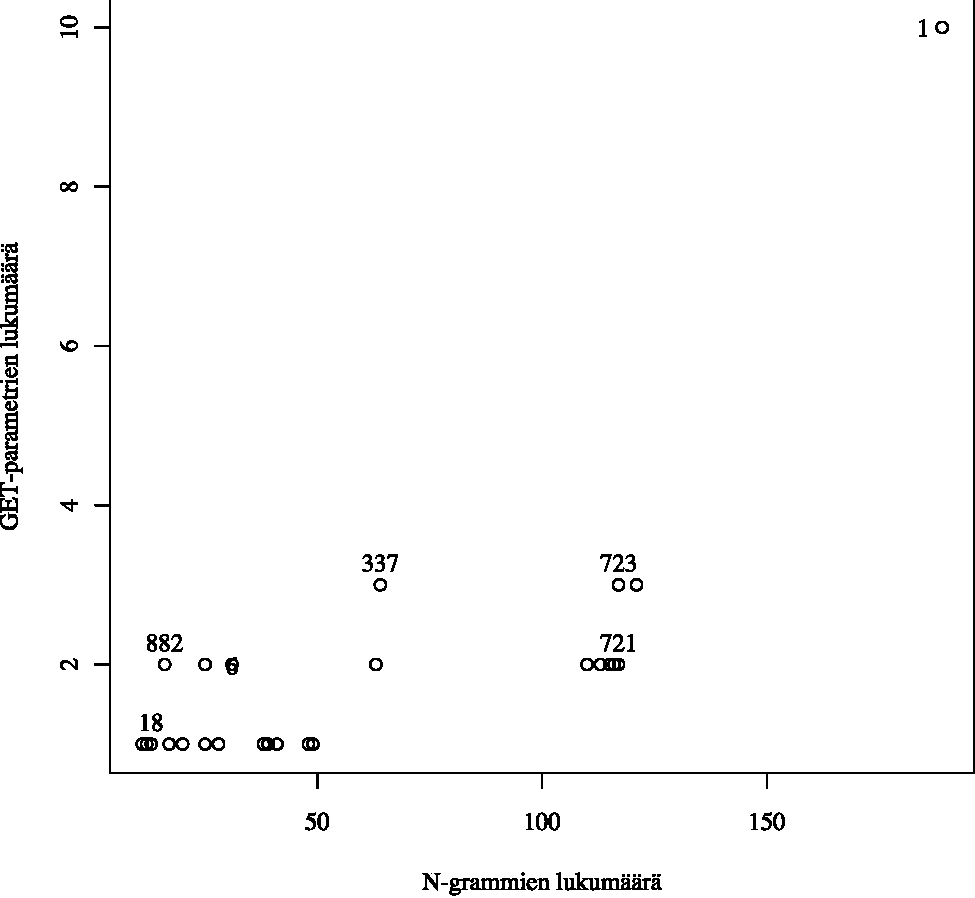
\includegraphics[width=13cm]{pics/service_resources.pdf}
\caption{Palvelun resurssien ominaisuudet.}
\label{service_resources}
\end{figure}

Analysoitavan palvelun eri resurssit on esitetty kuvassa
\ref{service_resources}. Kuvassa vaaka-\-akselina on käytetty
N-grammien lukumäärää ja pystyakselina GET-parametrien
lukumäärää. Resursseista valitsimme kuusi tarkempaan tarkasteluun ja
ne on merkitty kuvaajaan niiden resurssinumerolla.  Resurssit pyrimme
valitsemaan siten, että jokaisesta ryppäästä olisi yksi valittuna.

Palvelun jokaisesta resurssista muodostettiin aluksi diffuusiokuvaus
käyttäen edellä kuvatulla tavalla suodatettua aineistoa.
Analysoimalla saatua diffuusiokuvausta voitiin määrittää ne pisteet,
jotka oli luokiteltu poikkeaviksi siinä joukossa, jossa kyseisiä
pisteitä oli verrattu. 

Näin lasketuista diffuusiokuvauksista muodostettiin seuraavaksi
diffuusiokartta käytäen toista ja kolmatta ominaisvektoria. Koska
suuri määrä pisteitä sijoittui täsmälleen samoihin koordinaatteihin,
kartan luettavuuden parantamiseksi sirontakuvion pisteitä
``täristettiin''. Täristäminen suoritettiin lisäämällä
ominaisvektorien arvoihin normaalijakaumasta satunnaisesti poimittu
arvo. Normaalijakauman keskihajontana käytettiin yhtä prosenttia
akselin leveydestä. Kuvassa \ref{diffusio_1} nähdään edellä kuvatulla
tavalla muodostettu diffuusiokartta resurssista 1. Kuvaajasta voidaan
havaita, että muutamaa poikkeusta lukuunottamatta pisteet sijoittuivat
hyvin lähelle toisia.

Diffuusiokartta ei ole sellaisenaan kovinkaan havainnollinen, joten
jokaiselle pisteelle laskettiin vielä poikkeavuusluku. Se muodostettiin
summaamalla euklidinen etäisyys lähimpään kolmeen pisteeseen
diffuusiokuvauksen toisen, kolmannen ja neljännen ominaisvektorin
muodostamassa diffuusioavaruudessa. Tämän etäisyystiedon avulla voitiin piste
luokitella poikkeavuudeksi sekä piirtää poikkeavuuskartta.

% FIXME etäisyyskartta -> poikkeavuuskartta. Tuomon vinkki.

Kuvassa \ref{service_1} on resurssista 1 muodostettu poikkeavuuskartta. Kuvaajassa vaaka-akselille on sijoitettu resurssille kohdistuneet HTTP-kyselyt
ja pystyakselin mittana on poikkeavuus. Tässä pystyakseli ilmaisee sen kuinka poikkeava kukin piste on vertailujoukon sisällä. Jokaiselle kuvaajalle
on vielä määritetty keskihajonta ja raja-arvo, jonka ylittäneet pisteet merkitään poikkeaviksi. Tämä raja-arvo vaihtelee tapauskohtaisesti ja sen
arvo on kolme kertaa keskihajonta. Keskihajonta on merkitty kuvaajaan katkoviivalla ja raja-arvo yhtenäisellä viivalla. Esimerkiksi resurssin 1 
poikkeavuusskartassa \ref{service_1} on nähtävissä viisi poikkeavuudeksi merkittyä pistettä.

Jokainen diffuusiokartan luomiseen käytetytty piste pystytään
palauttamaan siihen HTTP-kyselyyn, josta se on
muodostettu. Esitetyissä kuvaajissa palauttamiseen tarvittavat tiedot
on merkitty niihin pisteisiin, jotka ylittävät raja-arvon. Otetaan
esimerkiksi kuvaajan \ref{service_18} ainoaksi merkitty poikkeama,
jolla on arvot ovat 7,3 ja 14594. Näistä ensimmäinen arvo ilmoittaa
sen tiedoston järjestysnumeron, josta kyseinen HTTP-kysely
löytyy. Seuraava luku puolestaan kertoo sen palvelimen
järjestysnumeron, johon kysely on ohjattu. Näiden kahden luvun avulla
voidaan yksilöidä tietty lokitiedosto. Viimeisin luku sisältää
rivinumeron kyseisen lokitiedoston sisällä.  Tämän kolmikon avulla
pystytään yksilöimään haluttu kysely ja pistettä vastaava alkuperäinen
palvelinlokin rivi voidaan löytää.

\section{Tulokset}

Analysoitavassa materiaalissa resurssilla 1 \ref{service_1} oli viisi HTTP-kyselyä, jotka merkittiin poikkeaviksi. Tutkimalla diffuusiokuvauksen
luomiseen käytettyä lokia, ja palauttamalla HTTP-kyselyt alkuperäiseen muotoon, pystyimme paikallistamaan nämä kyselyt ja vertaamaan niitä lokin
muihin kyselyihin. Resurssin 1 tapauksessa kolme poikkeavaksi merkittyä kyselyä sisälsi sellaisen tunnistetiedon käyttäjistä, jota ei esiintynyt 
muissa kyselyissä. Kahdesta jäljelle jääneestä kyselystä yhdessä oli yritetty suoraan pyytää sellaista sivustoa, johon palvelu ei todennäköisesti
tarjonnut mahdollisuutta. Viimeisin kysely sitten... FIXME: Tarkistettava Joelilta onko tuossa joku bugi?

Kuvassa \ref{service_18} on nähtävillä resurssin 8 poikkeavuuskartta. Kyseisessä otannassa oli mukana 181 pistettä ja näistä yksi todettiin poikkeavaksi.
Resurssi 8 tarjosi vain staattista sisältöä, joten GET-parametrin jälkeistä kyselyosuutta ei HTTP-kyselyissä pitänyt olla. Poikkeavassa kyselyssä oli
GET-parametrin resurssipolun jälkeen kuitenkin kysymysmerkki, ja tämän perässä oli pyynnön tehneen alustan verkko-osoite. Poikkeavan kyselyn tunnistaminen
oli helppoa, sillä se oli ainoa kysely, jolle n-gram analyysi tuotti rivejä. Resurssille tehty kysely oli selkeästi virheellinen, sillä merkitty verkko-osoite 
oli privaattiverkon osoite. Kyselyssä käytetty alusta oli myös ainoa laatuaan.

Resurssisa 337 \ref{service_337} poikkeavuuksia havaittiin kuusi kappaletta. Näistä neljässä oli GET-parametrin jälkeen lisättynä samanlainen tunnistetieto
kuin resurssin 1 kolmessa havaitussa poikkeavuudessa. Yksi poikkeavuus taas oli saman käyttäjän aiheuttama kuin resurssilla 8, sillä kysely tuli samasta
verkko-osoitteesta ja näiden välillä ei ollut kuin muutama minuutti aikaa. Käytetty alusta oli myös ainoa laatuaan ja kyselyyn oli lisätty perään
sama verkko-osoite. Onkin hyvin todennäköistä, että pyydetyt palvelut eivät ole suunniteltu kyseiselle alustalle, jolloin kyselyiden oikeassa muodostuksessa ilmenee
virheitä. Viimeisessä poikkeavassa kyselyssä oli sitten muista eroava määrä avain-arvo pareja.

Kuvien \ref{service_721} ja \ref{service_723} poikkeavuudet aiheutuivat samaan tapaan ylimääräisestä tunnistetiedosta, joka oli lisätty kyselyiden perään. Kyselyt olivat selkeästi tulleet
saman välityspalvelun kautta, ja niistä jokainen oli tullut eri käyttäjältä. Tämä viittaakin siihen, että kyseinen välityspalvelu on konfiguroitu virheellisesti jonka
takia sitä kautta tulevat pyynnöt eivät näy palvelimelle oikein. Viimeisessä kuvassa \ref{service_882} resurssin poikkeama aiheutui siitä, että kyseinen HTTP-pyyntö oli ainoa, johon oli lisätty erillinen arvo. 
Muut käyttäjät ainoastaan latasivat saman tiedostoa ilman ylimääräisiä parametreja.. 



\begin{figure}[p]
\centering
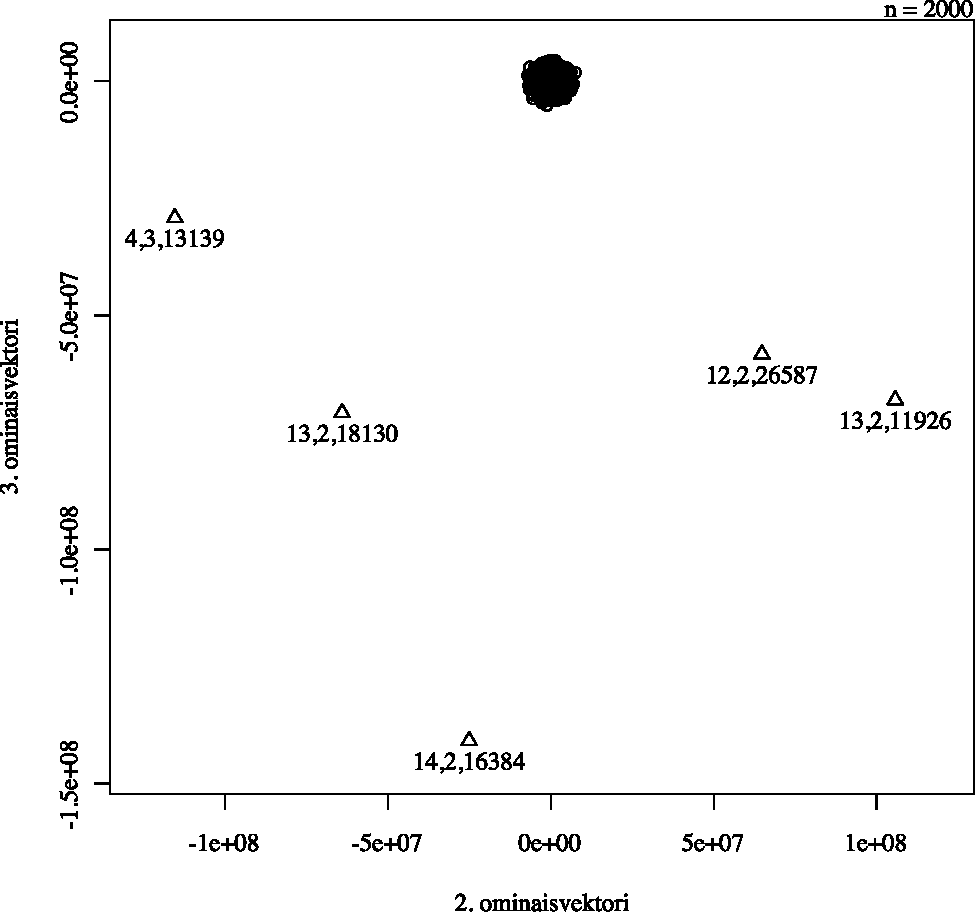
\includegraphics[width=11cm]{pics/diffuusiokuvat/service_1.pdf}
\caption{Resurssin 1 täristetty diffuusiokartta.}
\label{diffusio_1}
\end{figure}

\begin{figure}[p]
\centering
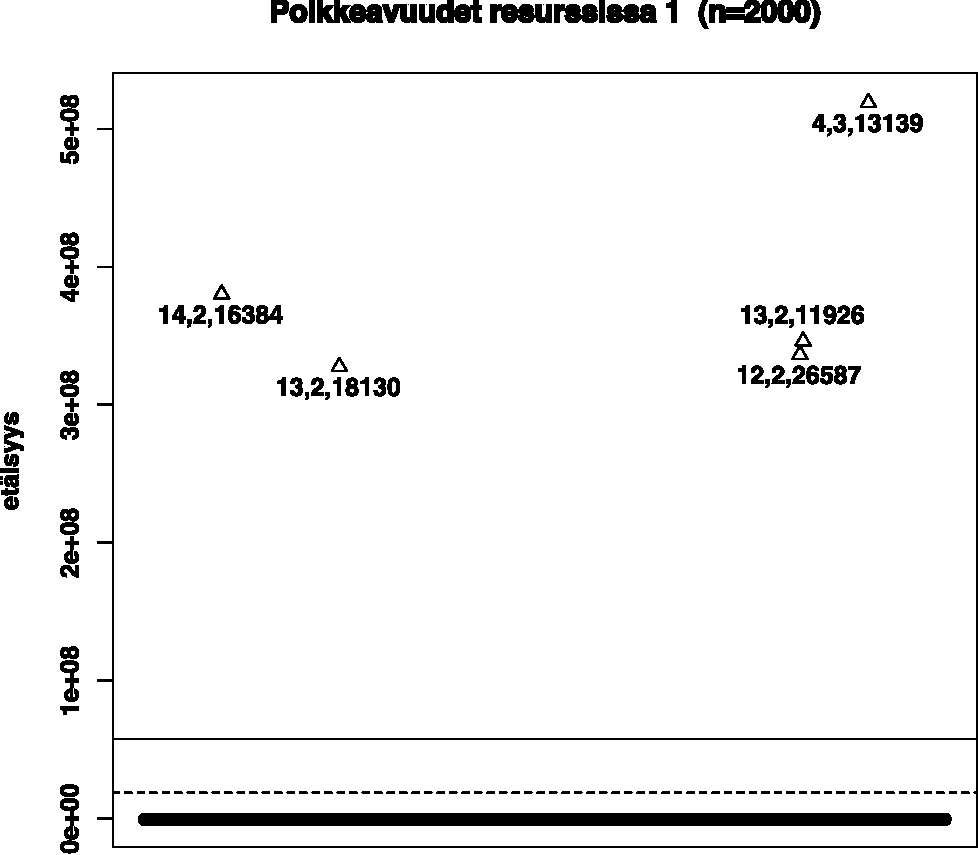
\includegraphics[width=11cm]{pics/tiheyskuvat/service_1.pdf}
\caption{Resurssin 1 poikkeavuuskartta.}
\label{service_1}
\end{figure}

\begin{figure}[p]
\centering
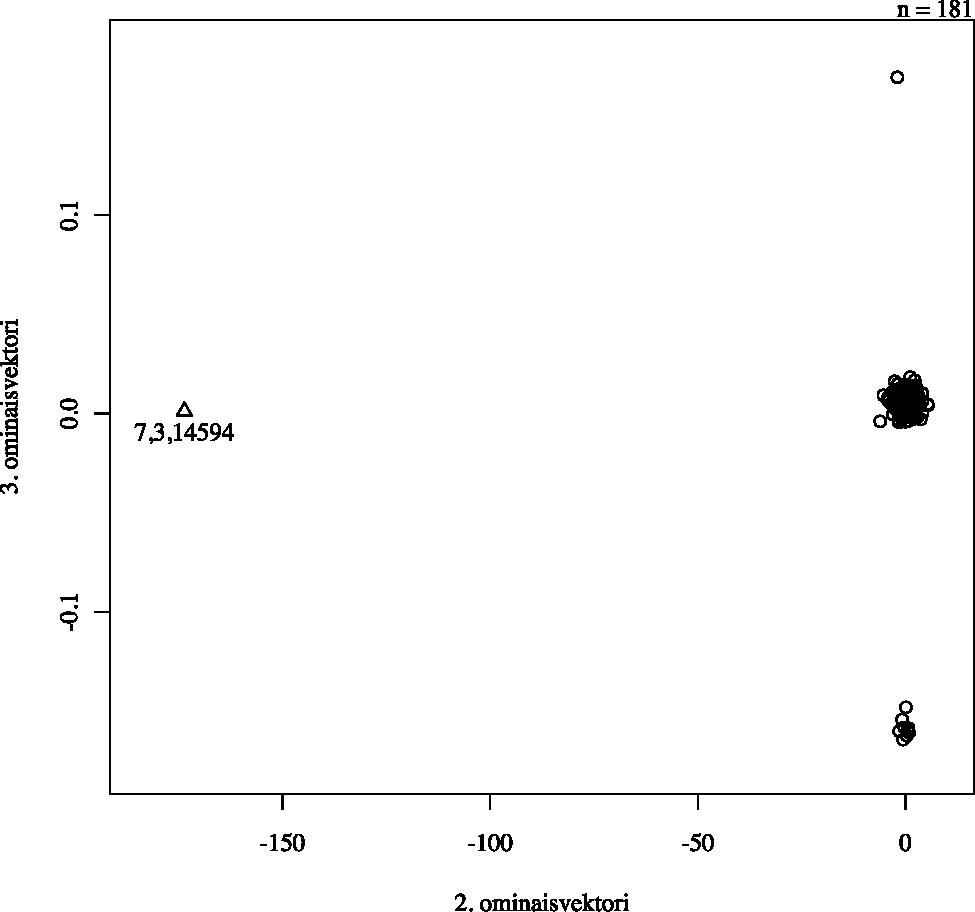
\includegraphics[width=11cm]{pics/diffuusiokuvat/service_18.pdf}
\caption{Resurssin 18 täristetty diffuusiokartta.}
\label{diffusio_18}
\end{figure}

\begin{figure}[p]
\centering
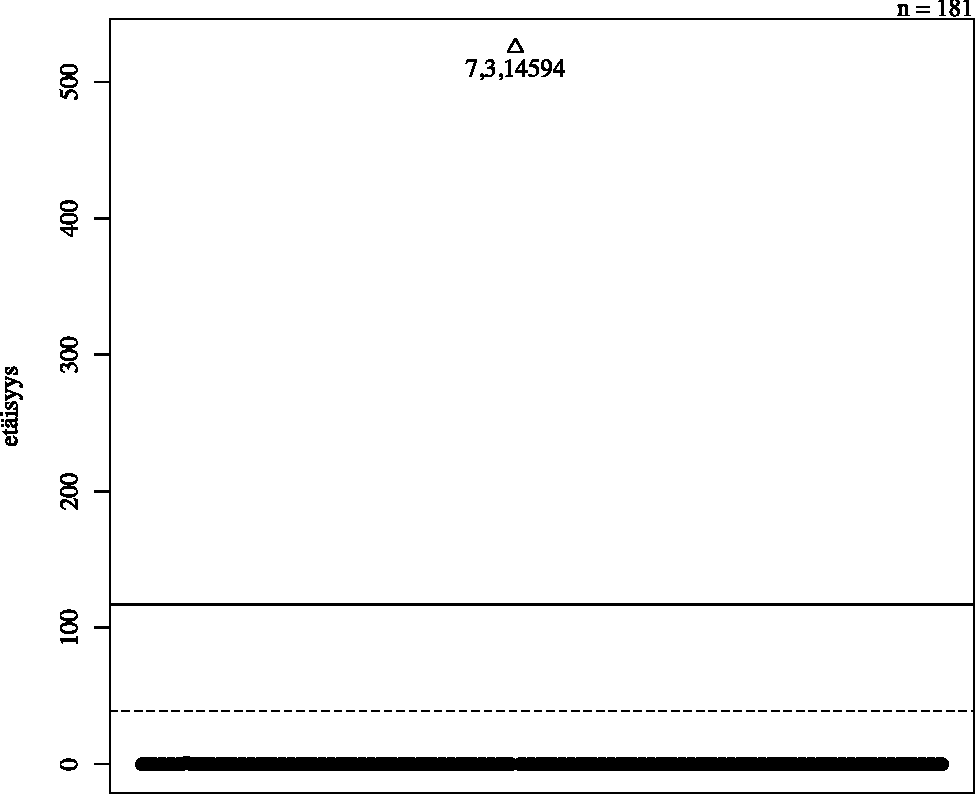
\includegraphics[width=11cm]{pics/tiheyskuvat/service_18.pdf}
\caption{Resurssin 18 poikkeavuuskartta.}
\label{service_18}
\end{figure}

\begin{figure}[p]
\centering
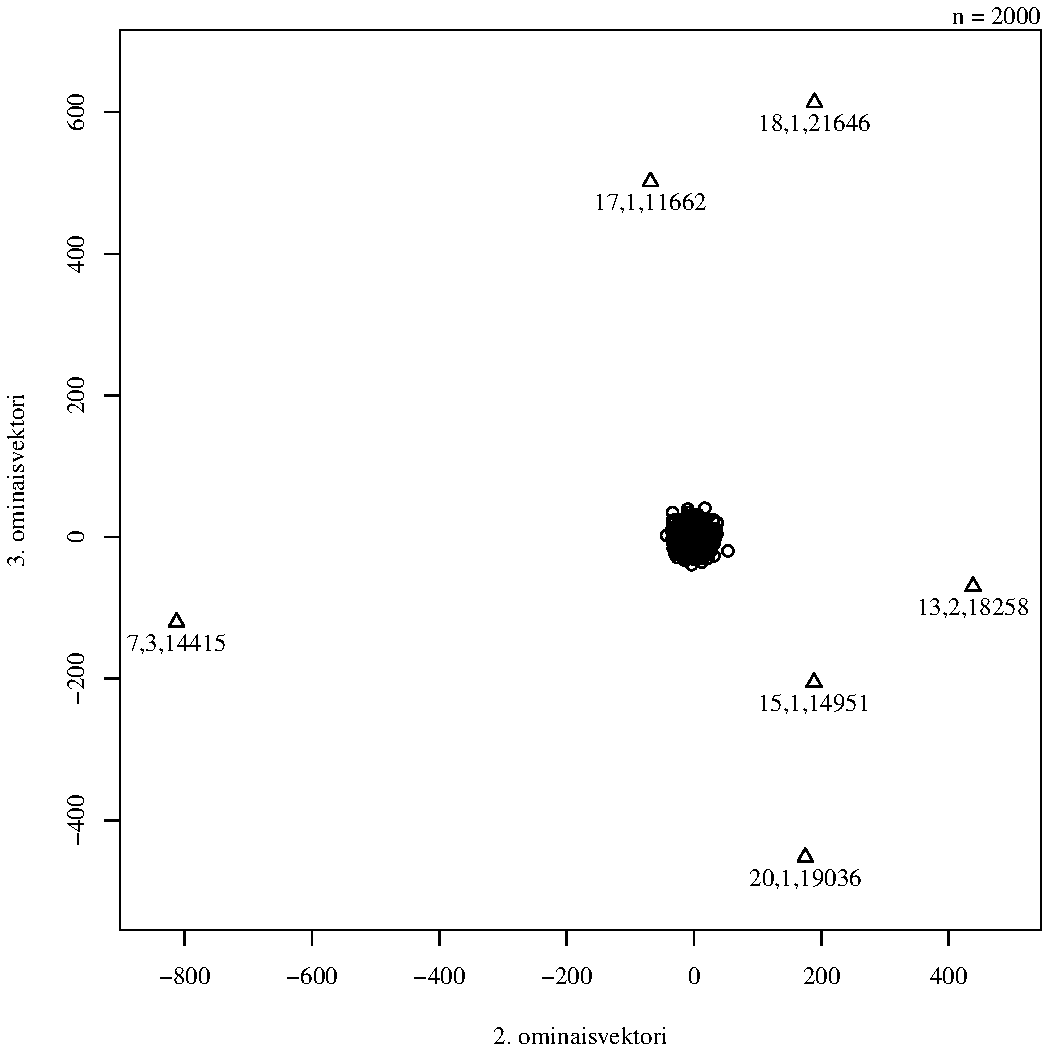
\includegraphics[width=11cm]{pics/diffuusiokuvat/service_337.pdf}
\caption{Resurssin 337 täristetty diffuusiokartta.}
\label{diffusio_337}
\end{figure}

\begin{figure}[p]
\centering
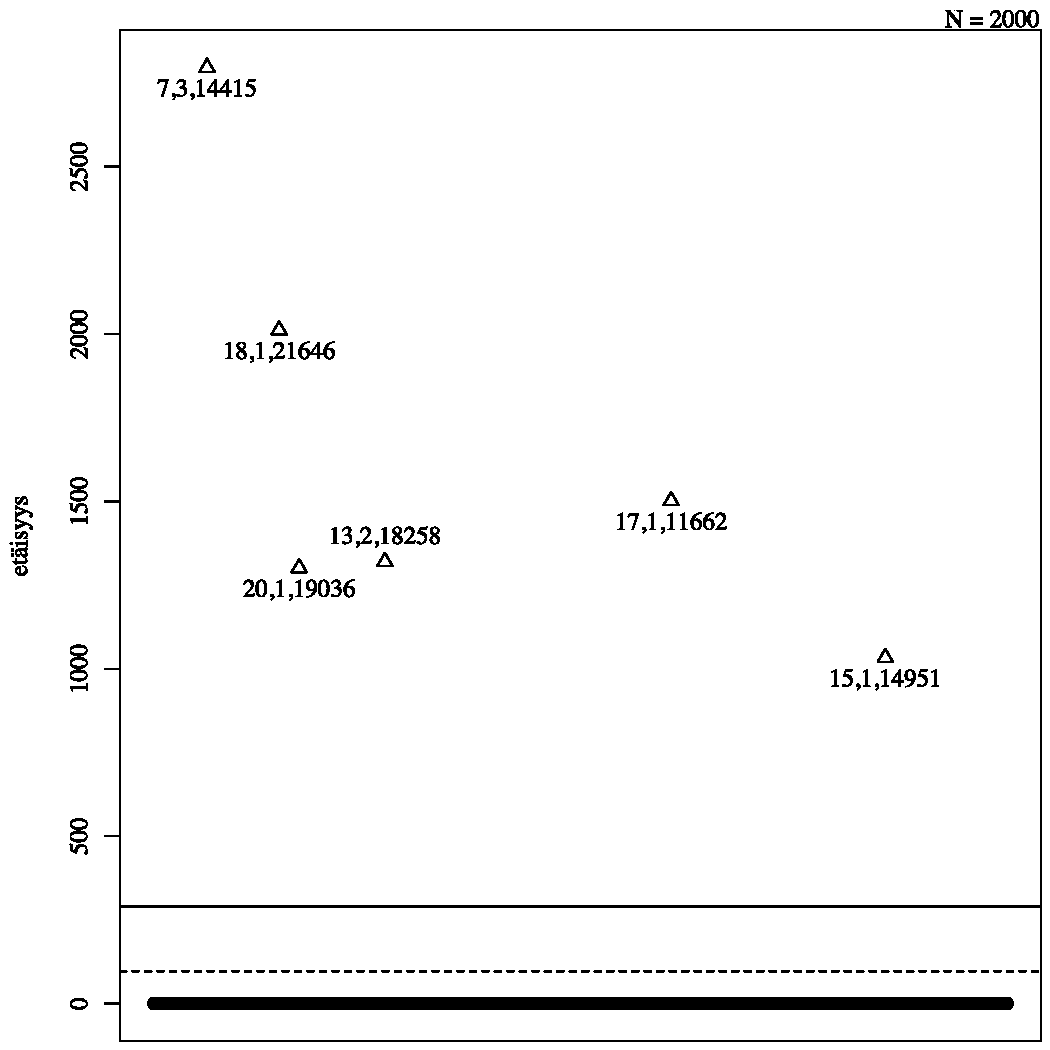
\includegraphics[width=11cm]{pics/tiheyskuvat/service_337.pdf}
\caption{Resurssin 337 poikkeavuuskartta.}
\label{service_337}
\end{figure}

\begin{figure}[p]
\centering
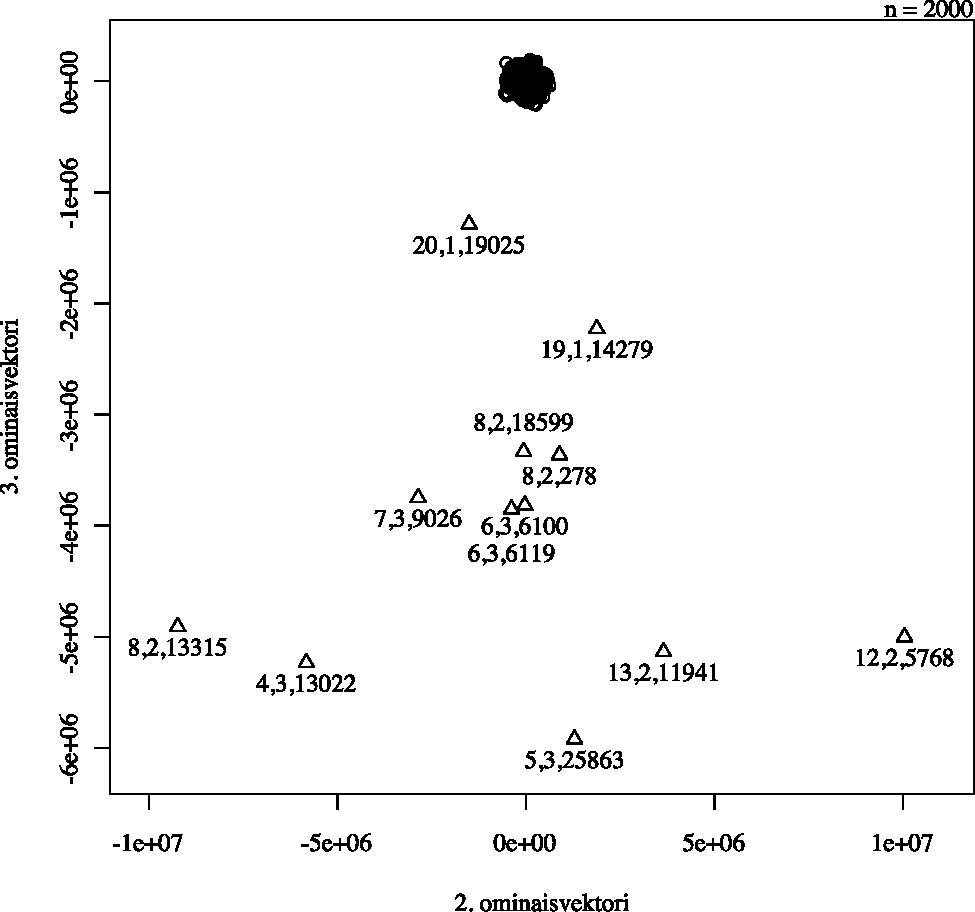
\includegraphics[width=11cm]{pics/diffuusiokuvat/service_721.pdf}
\caption{Resurssin 721 täristetty diffuusiokartta.}
\label{diffusio_721}
\end{figure}

\begin{figure}[p]
\centering
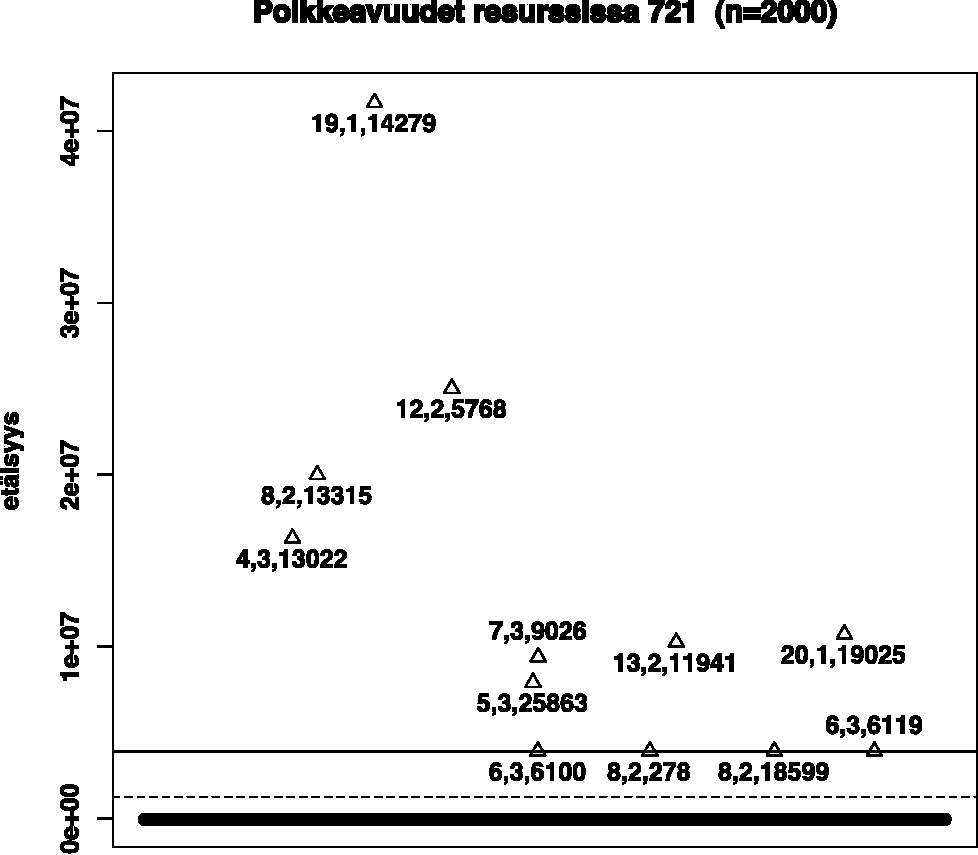
\includegraphics[width=11cm]{pics/tiheyskuvat/service_721.pdf}
\caption{Resurssin 721 poikkeavuuskartta.}
\label{service_721}
\end{figure}

\begin{figure}[p]
\centering
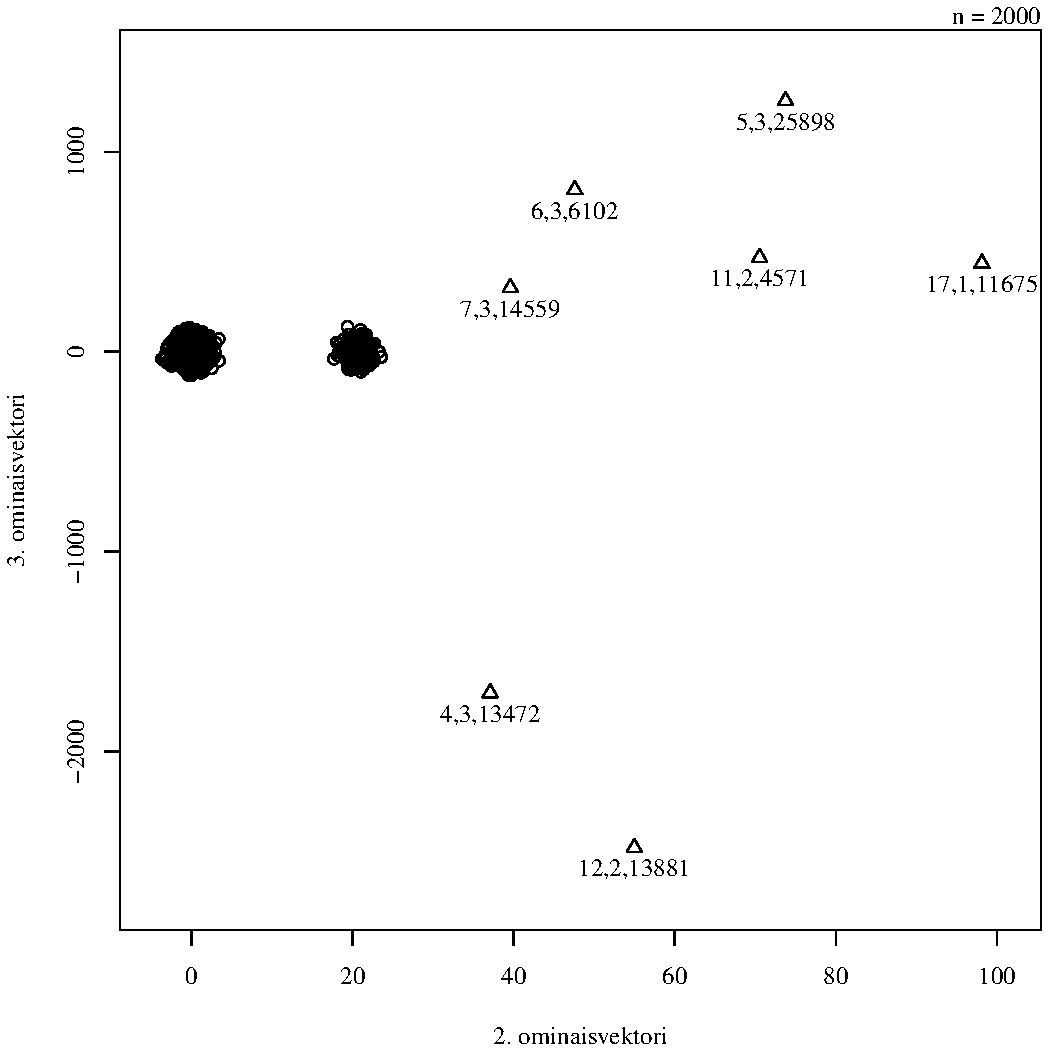
\includegraphics[width=11cm]{pics/diffuusiokuvat/service_723.pdf}
\caption{Resurssin 723 täristetty diffuusiokartta.}
\label{diffusio_723}
\end{figure}

\begin{figure}[p]
\centering
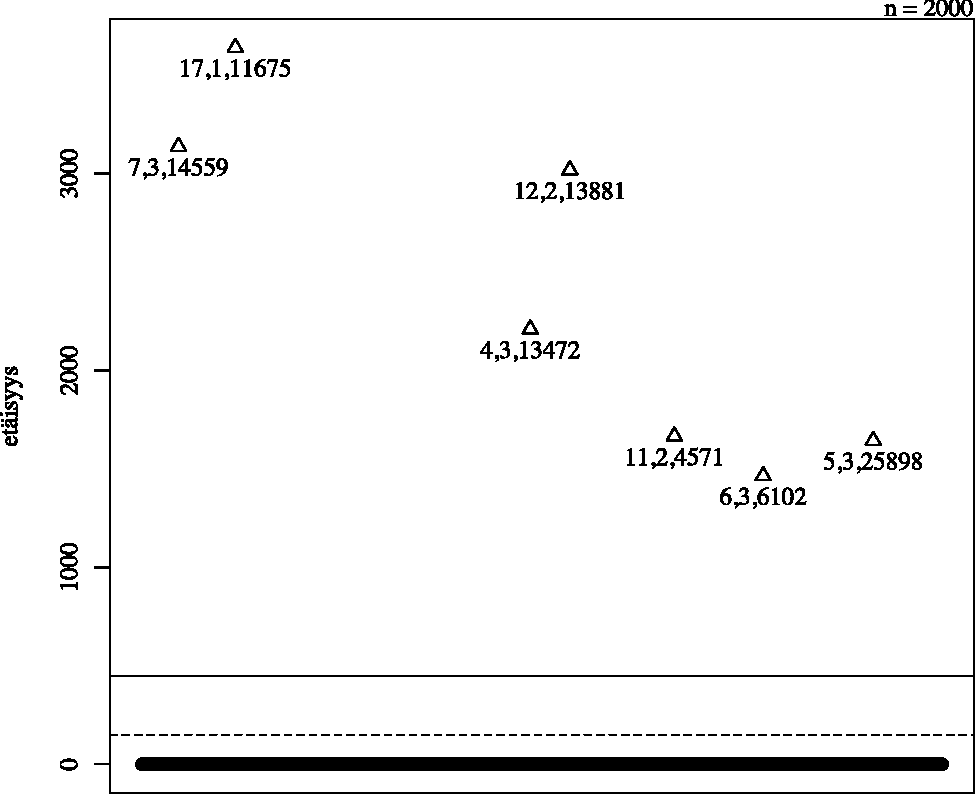
\includegraphics[width=11cm]{pics/tiheyskuvat/service_723.pdf}
\caption{Resurssin 723 poikkeavuuskartta.}
\label{service_723}
\end{figure}

\begin{figure}[p]
\centering
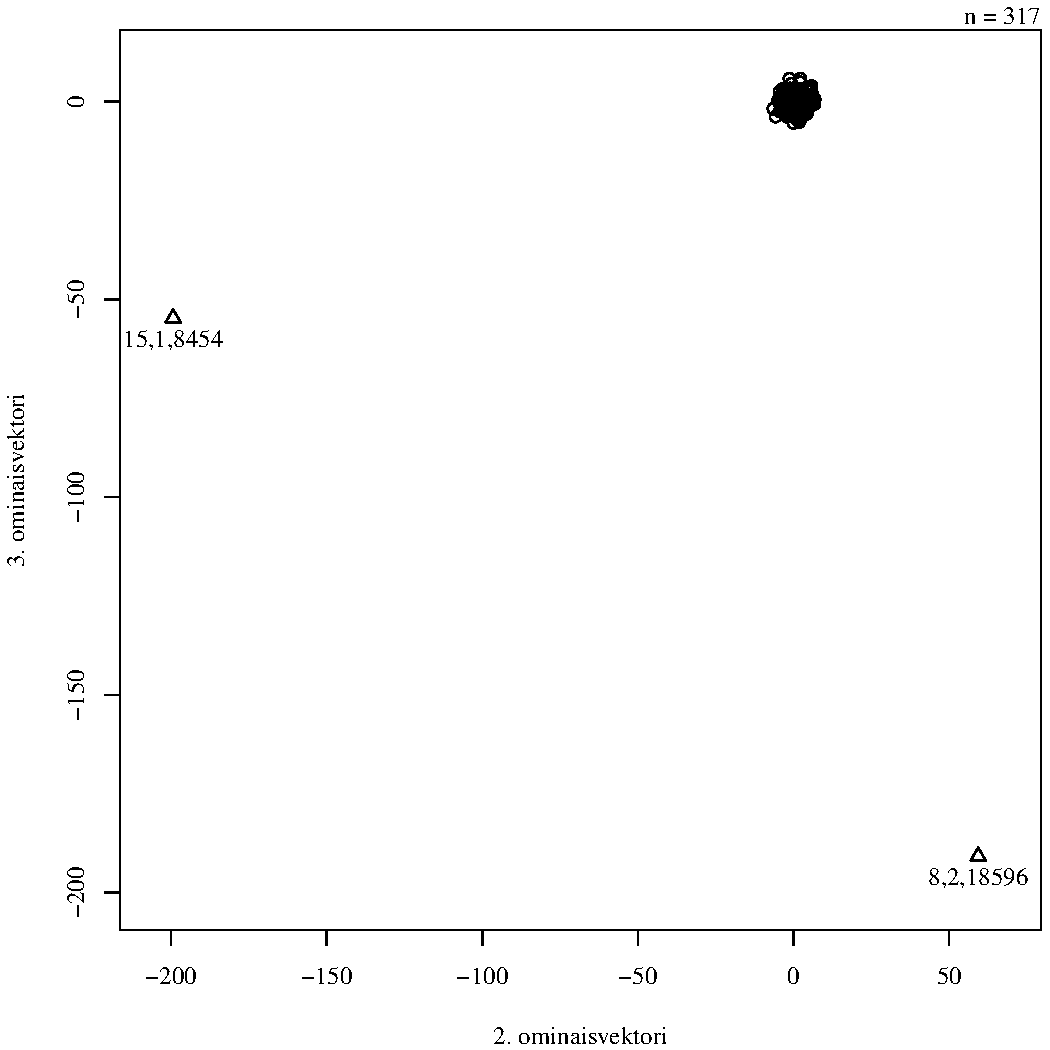
\includegraphics[width=11cm]{pics/diffuusiokuvat/service_882.pdf}
\caption{Resurssin 882 täristetty diffuusiokartta.}
\label{diffusio_882}
\end{figure}

\begin{figure}[p]
\centering
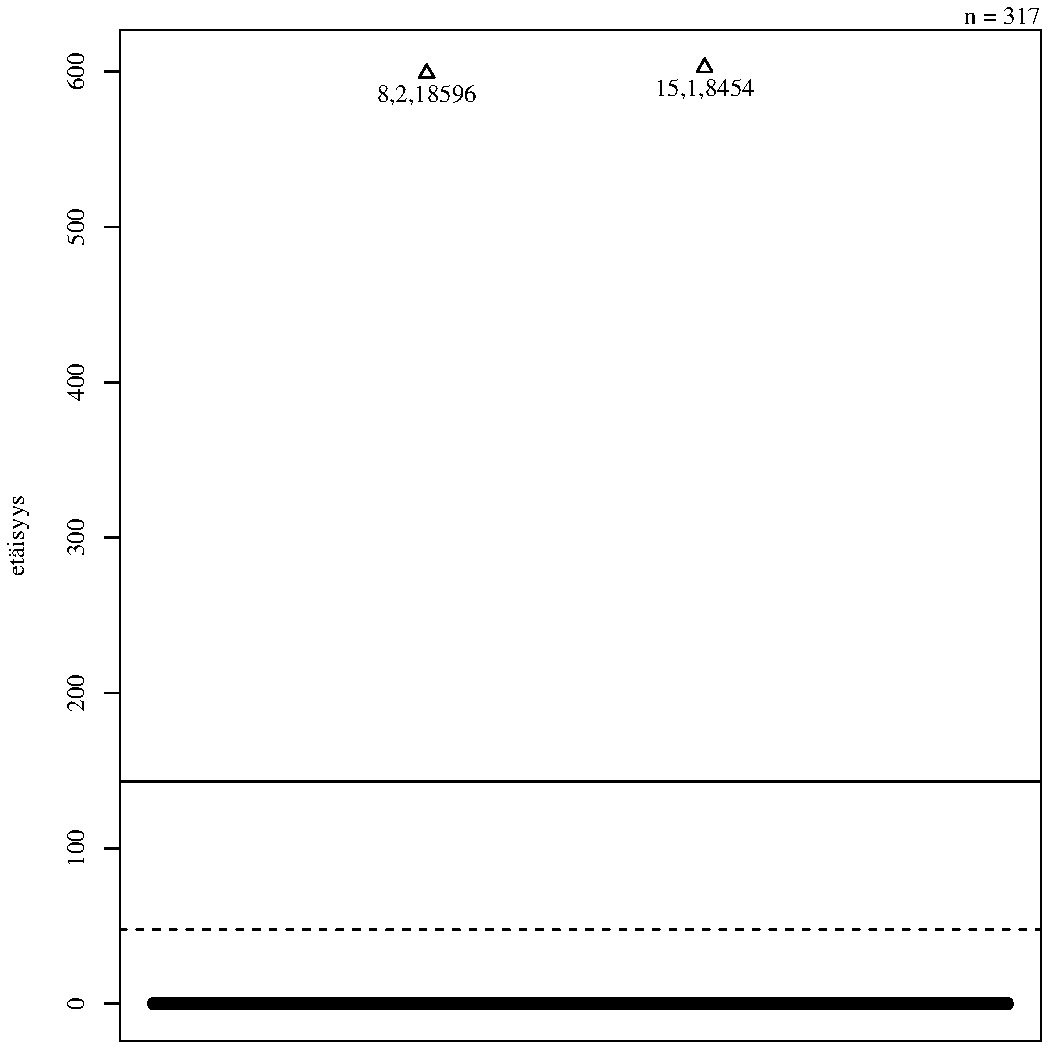
\includegraphics[width=11cm]{pics/tiheyskuvat/service_882.pdf}
\caption{Resurssin 882 poikkeavuuyskartta.}
\label{service_882}
\end{figure}

- Liikenne hyvin samakaltaista
- Verkkokerroksen hyökkäykset eivät näy logissa
- Mahdollisia aktiivisia palomuureja? verkon rakenne ei muutenkaan ole tarkkaan tiedossa
- Sisältävätkö kyseiset palvelut muutenkaan hyökkäysten kannalta kiinnostavia kohteita?


\section{Kehitysideoita}
% Keksi parempi otsikko? :-)

- Reaaliaikaisessa toteutuksessa aikavaativuus ei ole ongelma, koska järjestelmälle opetetaan etukäteen normaali käyttäytyminen, jonka jälkeen
uudet pisteet projisoidaan yksitellen kuvaan. Nyström extension

- Menetelmänt toimivuuden testauksen kannalta tarvittaisiin rajatumpaa materiaalia. Esimerkiksi lyhyempi ajan jakso sellaiselta hetkeltä, jolloin
 tiedetään hyökkäyksen tapahtuneen

- Opetusjakson määrittely

- Uusien parametrien määrittäminen. Onko tämä mahdollista? ESim. IP-osoite ja selaimen tunnistetieto
